\documentclass[10pt]{article}
\usepackage{icmlko}

\icmlmeta{IP 파운데이션 월드모델}{135}{팝업은 아무것도 판정하지 못한다}{노트 128부터 일곱 편에 걸쳐 ``제품 지표가 깎인다''고 적었다 --- 짝지어 재 보니 여섯 비교가 전부 탐지 한계 안이었다}

\begin{document}

\twocolumn[
\icmlheader

\begin{abstract}
노트 134가 ``판과 제품 지표가 반대로 움직인다, 결정이 필요하다''로 끝났다.
결정하기 전에 쟀다. \textbf{첫 수치는 그 말을 뒷받침했다} --- 고유 실행
27건에서 판 $\rho$와 팝업 $\rho$의 순위 상관이 $-$0.353이고, 축 세트로 봐도
정식화로 봐도 단조롭다. 축을 하나도 안 붙인 판이 팝업 최고($+$0.5436)이고
판 최저다. \textbf{그런데 짝지어 재니 아무것도 유의하지 않았다.} 팝업
$\rho$의 짝지은 차를 붓스트랩 2{,}000회로 재면 여섯 비교의 95\% 구간이
\emph{전부} 0을 가로지른다. 반폭이 0.06$\sim$0.16이고 내가 보고해 온
하락이 $-$0.045$\sim$$-$0.074다. \textbf{노트 128부터 일곱 편에 걸쳐 잡음을
신호로 읽었다.} 필요한 표본을 부분표집으로 직접 쟀다 --- 반폭 $=$
$1.03\,n^{-0.52}$이고, 0.05를 가르려면 $n\approx339$, 0.03이면
$n\approx905$다. \textbf{지금은 59다.} 지수 $-0.52$는 고전적인 $-0.5$와
사실상 같고, 이는 노트 123이 세운 $2.28\,n^{-0.88}$이 \emph{이 양에는}
안 맞는다는 뜻이다 --- 그 법칙으로 세운 표본 계획은 낙관적이었다. 발산의
절반은 판이 표본 수 가중이라 생긴다(큰 셋이 후행의 67\%, 팝업은 2.3\%).
비가중으로 바꾸면 $-$0.377이 $-$0.167로 준다. \textbf{남는 결론은 하나다.}
$n$=59에서 팝업은 목적함수로도 제약으로도 못 쓴다. 판과 제품이 갈리는지
아닌지조차 이 표본으로는 모른다.
\end{abstract}
]

\begin{figure*}[t]
\centering
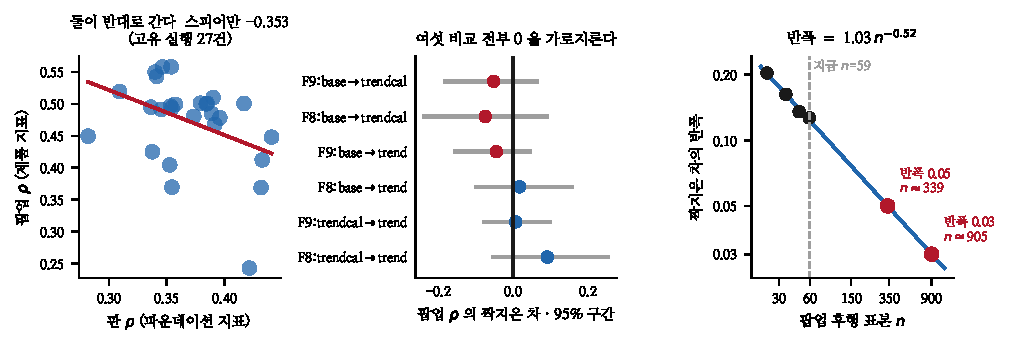
\includegraphics[width=\textwidth]{figs/power.pdf}
\caption{왼쪽 --- 실행 27건에서 판과 팝업이 반대로 간다. 가운데 --- 그런데
짝지은 차의 95\% 구간이 여섯 다 0을 가로지른다. 오른쪽 --- 부분표집으로
잰 필요 표본.}
\end{figure*}

\section{첫 수치는 발산을 뒷받침했다}

노트 128부터 축을 붙일 때마다 판이 오르고 팝업이 내렸다. 노트 134가 그것을
``미룰 수 없는 자리''로 적었다. 실행 기록 전부로 확인해 보니 정말 그렇게
보였다.

\begin{table}[t]
\centering\tsize
\caption{축 세트별 중앙값. 판 내림차순.}
\begin{tabular}{lrrr}
\toprule
& $n$ & 판 $\rho$ & 팝업 $\rho$ \\
\midrule
narrow\_trendcal & 2 & $+$.3932 & $+$.3694 \\
trend & 4 & $+$.3910 & $+$.5010 \\
wide\_trendcal & 2 & $+$.3872 & $+$.3237 \\
trend0 & 4 & $+$.3867 & $+$.4928 \\
trendcal & 6 & $+$.3655 & $+$.4872 \\
\textbf{base} & 7 & \textbf{$+$.3413} & \textbf{$+$.5436} \\
cal & 2 & $+$.3234 & $+$.4722 \\
\bottomrule
\end{tabular}
\end{table}

축을 하나도 안 붙인 \texttt{base}가 판 최저이면서 팝업 최고다. 정식화로
갈라도 같은 모양이다 --- 판 상위인 부스팅이 팝업 $+$0.4366이고, 판 하위인
결합 잠재 · 프로크루스테스가 팝업 $+$0.5584 · $+$0.5502다.

순위 상관이 $-$0.353(고유 실행 27건, 바닥선 제외 $-$0.446)이다.

\section{그런데 짝지어 재니 아무것도 없다}

여기서 멈추고 채택했으면 ``제품을 위해 축을 걷어내라''가 됐을 것이다.
대신 각 비교를 \emph{같은 표본에 짝지어} 붓스트랩했다.

\begin{table}[t]
\centering\tsize
\caption{팝업 $\rho$의 짝지은 차. 붓스트랩 2{,}000회, $n$=59.}
\begin{tabular}{lrr}
\toprule
& 차 & 95\% 구간 \\
\midrule
F9 base$\to$trendcal & $-$.0516 & [$-$.180, $+$.064] \\
F8 base$\to$trendcal & $-$.0739 & [$-$.236, $+$.091] \\
F9 base$\to$trend & $-$.0445 & [$-$.153, $+$.046] \\
F8 base$\to$trend & $+$.0176 & [$-$.097, $+$.157] \\
F9 trendcal$\to$trend & $+$.0072 & [$-$.077, $+$.098] \\
F8 trendcal$\to$trend & $+$.0916 & [$-$.053, $+$.253] \\
\bottomrule
\end{tabular}
\end{table}

\claimx{\textbf{여섯 다 0을 가로지른다.} 반폭이 0.06$\sim$0.16이고 내가
보고한 하락이 $-$0.045$\sim$$-$0.074다. \textbf{노트 128 · 129 · 130 ·
131 · 132 · 133 · 134에서 ``팝업이 내린다''고 적은 것은 전부 탐지 한계
안이었다.}}{순위 상관 $-$0.353 자체는 27건을 모은 값이라 다른 통계량이다.
다만 그 27건이 서로 독립이 아니고(같은 자료 · 겹치는 설정) 표준오차가
0.20쯤이라, 그것도 확립됐다고 하기 어렵다.}

\section{그러면 몇 건이 필요한가}

노트 123이 세운 구간 법칙 $2.28\,n^{-0.88}$이 있지만 그것은 채택 기준의
짝지은 차를 재고 만든 것이라 이 양에 그대로 쓸 수 없다. 직접 쟀다 ---
지금의 59건을 부분표집해 반폭이 $n$에 따라 어떻게 주는지 본다.

\begin{table}[t]
\centering\tsize
\caption{부분표집. F9 · base$\to$trendcal.}
\begin{tabular}{rr}
\toprule
$n$ & 반폭 \\
\midrule
23 & .2039 \\
35 & .1629 \\
47 & .1354 \\
59 & .1269 \\
\bottomrule
\end{tabular}
\end{table}

\claimx{\textbf{반폭 $=$ $1.03\,n^{-0.52}$.} 0.05를 가르려면
$n\approx339$, 0.03이면 $n\approx905$다. 지금은 59다.}{지수 $-0.52$가
고전적인 $-0.5$와 사실상 같다. \textbf{그러므로 노트 123의 $-0.88$은 이
양에 안 맞는다} --- 그 법칙은 표본을 늘리면 훨씬 빨리 좁아진다고 말하고,
그 말로 세운 계획(``476건이면 $\pm$0.010'')은 이 양에 대해 낙관적이었다.}

\section{발산의 절반은 가중 때문이다}

판은 대상별 $\rho$를 채점 표본 수로 가중 평균한다. 후행 2{,}614건 중
웹툰 · 애니 · 모바일이 1{,}758건(67.3\%)이고 팝업은 59건(2.3\%)이다.

\claimx{\textbf{비가중으로 바꾸면 발산이 절반으로 준다} --- 판과 팝업의
순위 상관이 $-$0.377에서 $-$0.167이 된다. 나머지 절반은 팝업이 실제로
다른 도메인과 다르게 움직이는 몫이다.}{$-$0.167도 유의한지는 위와 같은
이유로 모른다. 그리고 비가중 평균은 표본이 작은 도메인의 잡음을 그대로
받아들이므로 판정 지표로는 더 나쁘다.}

\section{남는 결론}

\claimx{\textbf{$n$=59에서 팝업은 목적함수로도 제약으로도 못 쓴다.}
목적함수로 쓰기엔 귀무 폭이 $\pm$0.26이고(노트 125), 제약으로 쓰기엔
탐지 한계가 $\pm$0.13이다. 판이 제품을 깎고 있는지 아닌지조차 이 표본으로는
모른다.}{``모른다''가 ``안 깎는다''는 아니다. 판을 순위 기준으로 계속
쓰되, 팝업 수치는 \emph{보고는 하고 판정에는 안 쓰는} 것으로 명시한다.}

\begin{table}[t]
\centering\tsize
\caption{남은 것.}
\begin{tabular}{ll}
\toprule
표본 & 팝업 후행 59 $\to$ 339 이 유일한 길 \\
가드 & 탐지 한계 아래 차이를 서술하지 말 것 \\
노트 123 & $n^{-0.88}$ 법칙의 적용 범위를 좁힐 것 \\
\bottomrule
\end{tabular}
\end{table}

둘째 줄은 이 노트가 만든 규칙이다. 일곱 편에 걸쳐 반폭 안의 차이를 문장으로
서술했다. 수치를 적는 것과 \emph{그 수치로 이야기를 만드는 것}은 다르고,
후자에는 구간이 필요하다. \textbf{앞으로 팝업 차이는 짝지은 구간과 함께
적거나 아예 적지 않는다.}

\end{document}
